\chapter{Schedule}
In this part, we are going to treat the organization of the team on this project. To begin, we identified the various tasks which will constitute this project. Thanks to elements identified previously, we made a diagram of Gantt which is a tool used in project management, and allowing the affectation of a task for one person or a group of person, the time which this task will have to take. He allows to visualize the fulfillment of the tasks according to time.
\section{Tasks List}
A list of task was identified from the beginning by the project to be able to lead it most effectively possible from the beginning to the end.
\begin{itemize}
\item The choice of the subject. We took a subject which concerned drones because the majority of our team follow the subject Communicating Autonomous Systems.
\item An analysis of existing concerning the communicating autonomous systems. We read about ten articles in touch with our main subject.
\item An update of various articles previously studied is essential. Indeed, the speed of evolution of the technology today is so important that a written article two or three years ago may be out of date.
\item The development of both present models in the studied article.
\item The writing of this report.
\item The preparation of the orals.\\
\end{itemize}

\section{GANTT}
\begin{figure}[h]
\center
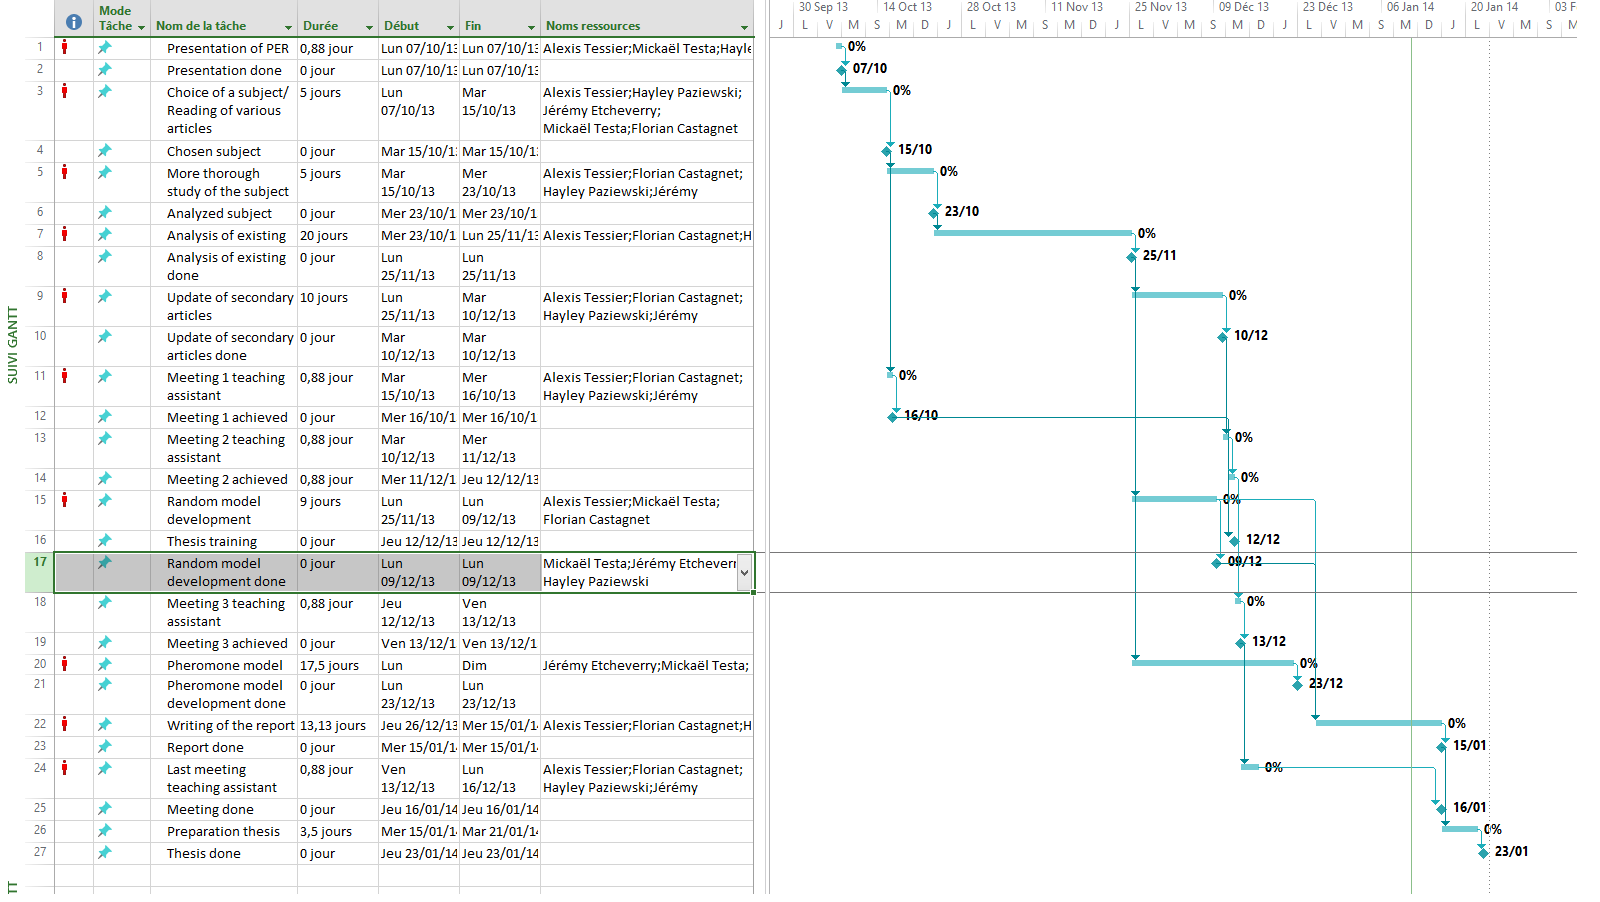
\includegraphics[scale=0.7]{../images/Gantt.png}
\caption{\label{Gantt}Diagram of Gantt of our project}
\end{figure}